
This chapter describes the work done in each sprint. A sprint is one iteration
of the Scrum process (see section \ref{section:scrum} for more information about
Scrum). The duration of each sprint was two weeks. Every sprint was assigned
various tasks from the project backlog. Each task was given a specific point
value and assigned to one or more team members. The point value is an estimation
of the amount of work (measured in man-hours) that is required to complete the
task. The point value can be also influenced by the importance of the task.
If a task required more time than planned and was not finished by the end of
the sprint, it was assigned a 'prolonged' status and moved to the next sprint.

For table layout reasons we used some name abbreviations for the names
of task assignees.

\begin{table}[ht!]
\begin{tabular}{ | c | l | }

\hline
\textbf{Abbreviation} & \textbf{Name} \\
\hline

 AN & \anders	\\
\hline
 AS & \asbjorn	\\
\hline
 B  & \bjornar	\\
\hline
 E  & \emanuele	\\
\hline
 JH & \johan	\\
\hline
 JN & \jonas	\\
\hline
 H  & \henrik	\\
\hline

\end{tabular}
\end{table}

\newpage

\section{Sprint 1}

Duration: 20/01 to 02/02
Points total: 91

The first sprint was dedicated to planning meetings and working hours
and studying about interested technologies. While some team members had some
experience with Arduino, none of us had any experience with Android application
development and social networks. Each member chose his own role in the project,
based on his own area of interest. The team did a lot of brainstorming in
order to identify possible product ideas to show the customer and produced a
small proof-of-concept application. The meeting with the customer was arranged
for the beginning of the second week.

\begin{table}[ht!]
\begin{tabular}{ | r | l | c | c | r | }

\hline
\textbf{ID} & \textbf{Task} & \textbf{Points} & \textbf{Assigned to} & \textbf{Status} \\
\hline

 7 & Brainstorm ideas about the product		& 18 & Everyone		& done \\
\hline
 8 & Search for similar products			& 14 & Everyone		& done \\
\hline
 9 & Proof-of-concept application			& 12 & AN,B,E,JH	& done \\
\hline
12 & Read on OpenSocial						& 10 & E,H,JN		& done \\
\hline
13 & Read on Arduino						& 8  & AN,AS,B,JH	& done \\
\hline
11 & Read Facebook developers' pages		& 8  & E			& done\\
\hline
10 & Choose a development process			& 6  & Everyone		& done \\
\hline
 6 & Meet with the customer					& 4  & Everyone		& done \\
\hline
10 & Read on development processes			& 4  & Everyone		& done \\
\hline
 2 & Plan group meetings					& 2  & Everyone		& done \\
\hline
 5 & Plan meetings with the customer		& 2  & Everyone		& done \\
\hline
 1 & Exchange contact information			& 1  & Everyone		& done \\
\hline
 4 & Setup mailing list						& 1  & JN			& done \\
\hline
 3 & Setup a Skype chat						& 1  & JH			& done \\
\hline

\end{tabular}
\end{table}

\newpage

\begin{figure}[h!]
\centering 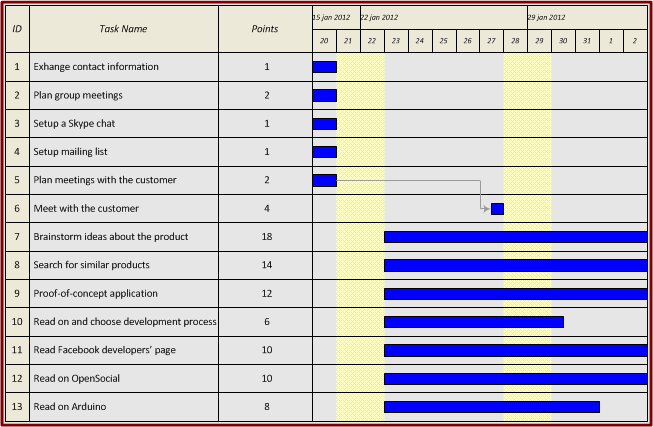
\includegraphics[scale=0.8]{img/sprints-gantt1.png}
\caption{Gantt diagram for the first sprint}
\label{fig:sprints-gantt1}
\end{figure}

\newpage


\section{Sprint 2}

Duration: 03.02 to 16.02
Points total: 100

The second iteration was focused on producing more prototypes of the product to
show the customer in order to receive the necessary feedback to identify
the product requirements and to begin designing the different parts of the
system, as well as acquiring the necessary knowledge and confidence with the
involved technologies. The team also worked on the preliminary version of the
report. The customer suggested that in order to show the re-usability
capabilities of the code, two more prototypes, considerably simpler than the
T-shirt prototype, could be produced for the project.

\begin{table}[ht!]
\begin{tabular}{ | r | l | c | c | r | }

\hline
\textbf{ID} & \textbf{Task} & \textbf{Points} & \textbf{Assigned to} &\textbf{Status} \\
\hline

 2 & Delivery of preliminary report				& 24 & Everyone		& done \\
\hline
 1 & Present a working prototype (week 1)		& 18 & Everyone		& done \\
\hline
 6 & Study Android application development		& 18 & Everyone		& done \\
\hline
 7 & Study Facebook Android SDK					& 12 & E			& done \\
\hline
 3 & Present a working prototype (week 2)		& 8  & Everyone		& done \\
\hline
 4 & Bluetooth connection to Arduino			& 8  & AN,JH		& done \\
\hline
 5 & Connect to Facebook (Facebook SDK)			& 6  & E			& done \\
\hline
 8 & Setup ScrumDo								& 1  & AN			& done \\
\hline
 9 & Setup GIT repository						& 1  & JN			& done \\
\hline

\end{tabular}
\end{table}

\begin{figure}[h!]
\centering 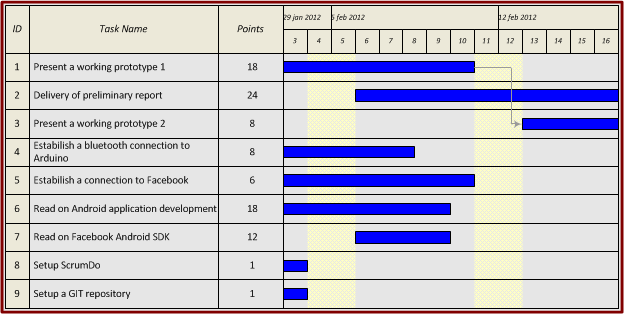
\includegraphics[scale=0.8]{img/sprints-gantt2.png}
\caption{Gantt diagram for the second sprint}
\label{fig:sprints-gantt2}
\end{figure}

\newpage

\section{Sprint 3}

Duration: 17.02 to 01.03
Points total: 108

This sprint was focused on proceeding with the design using the customer
feedback on the prototypes presented. An initial version of the Communication
library was also designed and coded. Design of the Social library also began.
During this sprint the system design started to take shape, and the various
parts of the system became more definite. The team delivered a list of hardware
needed to build the various T.U.I. prototypes. The customer was happy with the
team work so far and provided very valuable feedback.

\begin{table}[ht!]
\begin{tabular}{ | r | l | c | c | r | }

\hline
\textbf{ID} & \textbf{Task} & \textbf{Points} & \textbf{Assigned to} & \textbf{Status} \\
\hline

 4 & Social library design (part I)					& 20 & E		& done \\
\hline
 5 & Comm. library design (part I)			& 20 & AN,JH	& done \\
\hline
 1 & Present a working prototype (week 1)			& 18 & Everyone & done \\
\hline
 6 & Comm. library coding (part I)			& 16 & AN,JH	& done \\
\hline
 3 & Initial system design							& 14 & E,H		& done \\
\hline
 7 & Read on Android IPC mechanisms					& 12 & E		& done \\
\hline
 2 & Present a working prototype (week 2)			& 8 & Everyone	& done \\
\hline

\end{tabular}
\end{table}

\begin{figure}[h!]
\centering 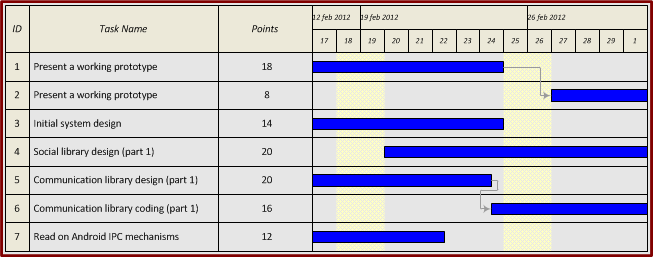
\includegraphics[scale=0.8]{img/sprints-gantt3.png}
\caption{Gantt diagram for the third sprint}
\label{fig:sprints-gantt3}
\end{figure}

\newpage


\section{Sprint 4}

Duration: 02.03 to 15.03
Points total: 112

This sprint was mainly aimed to the delivery of the mid-term report as well
as polishing of the Communication library. The design of the Social library
couldn't be completed in time due to design issues. The team had a hard
time trying to find a satisfying solution. These issues were presented to the
customer who provided valuable feedback that helped solve them.

\begin{table}[ht!]
\begin{tabular}{ | r | l | c | c | r | }

\hline
\textbf{ID} & \textbf{Task} & \textbf{Points} & \textbf{Assigned to} & \textbf{Status} \\
\hline

 1 & Work on the report				& 24 & Everyone & done \\
\hline
 2 & Present a working prototype	& 18 & Everyone & done \\
\hline
 3 & System design					& 18 & E 		& done \\
\hline
 7 & Comm. library coding (part II)	& 16 & AN,JH	& done \\
\hline
 4 & Social libray design (part II)	& 14 & E,H		& prolonged \\
\hline
 6 & Comm. library design (part II)	& 12 & AN,JH	& done \\
\hline
 5 & Social library coding (part I)	& 10 & E 		& done \\
\hline

\end{tabular}
\end{table}

\begin{figure}[h!]
\centering 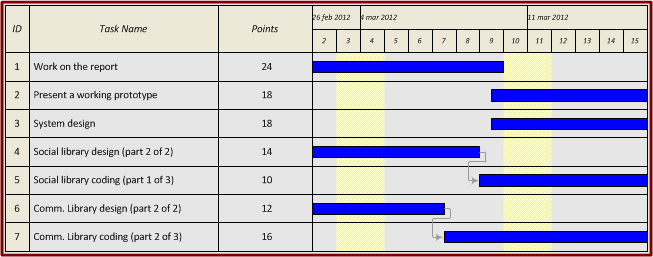
\includegraphics[scale=0.8]{img/sprints-gantt4.png}
\caption{Gantt diagram for the fourth sprint}
\label{fig:sprints-gantt4}
\end{figure}

\newpage

\section{Sprint 5}

Duration: 16.03 to 29.03
Points total: 128

During this sprint the team produced yet another prototype for the customer
and proceeded with the design and coding of the Social library. Coding of the
Communication library also continued, and an initial version was deployed by the
end of the sprint. The team also did some brainstorming and identified the other
two prototypes that were to be presented together with the T-shirt. Some
proof-of-concept applications for these prototypes were also made. This sprint
was a bit more intensive than the previous ones to cope with the fact that the
next sprint would have coincided with Easter vacation. The team still had not
received the hardware needed in order to begin building the T-shirt
prototype.

\begin{table}[ht!]
\begin{tabular}{ | r | l | c |c | r | }

\hline
\textbf{ID} & \textbf{Task} & \textbf{Points} & \textbf{Assigned to} & \textbf{Status} \\
\hline

 2 & Social library design (part II)			& 24 & E 		& completed \\
\hline
 4 & Comm. library coding (part III)	& 22 & AN,JH	& done \\
\hline
 3 & Social library coding (part II)			& 20 & E		& done \\
\hline
 1 & Present a working prototype				& 18 & Everyone	& done \\
\hline
 5 & Deploy the Comm. library					& 14 & JH		& done \\
\hline
 7 & Temperature prototype coding (part I)		& 10 & B 		& done \\
\hline
 9 & Led prototype coding (part I)				& 10 & AS 		& done \\
\hline
 6 & Temperature Prototype research				& 6  & B 		& done \\
\hline
 8 & Led prototype research						& 4  & AS 		& done \\
\hline


\end{tabular}
\end{table}


\begin{figure}[h!]
\centering 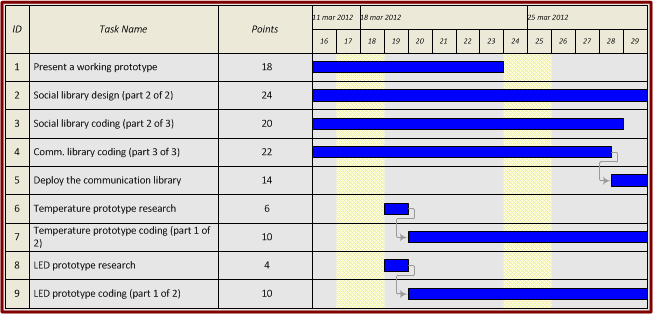
\includegraphics[scale=0.8]{img/sprints-gantt5.png}
\caption{Gantt diagram for the fifth sprint}
\label{fig:sprints-gantt5}
\end{figure}


\newpage

\section{Sprint 6}

Duration: 30.03 to 12.04
Points total: 50

As this sprint coincided with Easter vacation, little was planned for this
sprint except some early work on the report and some coding for the Social
library and the second prototype. Some team members left the city, others left
the country. No meetings with the customer were arranged. The team had a brief,
sort of 'unplanned' meeting right before the vacation during which they were
told that the hardware hadn't yet been ordered.

\begin{table}[ht!]
\begin{tabular}{ | r | l | c | c | r | }

\hline
\textbf{ID} & \textbf{Task} & \textbf{Points} & \textbf{Assigned to} & \textbf{Status} \\
\hline

1 & Work on the report					& 18 & Everyone & done \\
\hline
2 & Social library coding (part III)	& 16 & E		& done \\
\hline
3 & Temperature prototype coding (II)	& 16 & B		& done \\
\hline

\end{tabular}
\end{table}

\begin{figure}[h!]
\centering 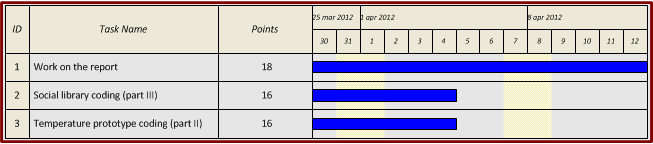
\includegraphics[scale=0.8]{img/sprints-gantt6.png}
\caption{Gantt diagram for the sixth sprint}
\label{fig:sprints-gantt6}
\end{figure}

\newpage

\section{Sprint 7}

Duration: 13.04 - 27.04
Points total:

Back from Easter vacation! Roughly one week after the group was back from
Easter vacation, the necessary hardware components needed for the product had
arrived. Also Mr. Babak, the customer, kindly provided a jacket that was to be
used for the final product.

The various hardware devices were hooked up with the Lilypad board and
then tested individually, using a mockup application.

During this sprint the final product changed sightly from a T-shirt to a jacket.
The Lilypad board probably wasn't the best choice for a jacket product, in fact,
since the Arduino board could be hidden in a pocket, the team could have used
a smaller Arduino board, maybe with power connector and built-in battery
charger circuitry.

The Social library was finished, tested and an initial version deployed.
The Comm. lib started being thouroghly tested along with the prototypes.

Coding for the T-shirt application began.

The Facebook and Twitter application started being converted from simple
mockups to complete applications.




\begin{table}[ht!]
\begin{tabular}{ | r | l | c | c | r | }

\hline
\textbf{ID} & \textbf{Task} & \textbf{Points} & \textbf{Assigned to} & \textbf{Status} \\
\hline


2 & T-Shirt application coding (part I)			& 22 & H			& done \\
\hline
1 & Build the T-shirt prototype (part I)		& 18 & AN,E,JH	& done \\
\hline
3 & Comm. library testing (part I)				& 16 & AN,E,JH	& done \\
\hline
4 & Temperature prototype testing	(part I)	& 16 & B			& done \\
\hline
6 & Work on report								& 14 & Everyone		& done \\
\hline
4 & Social library testing (part I)				& 12 & E,H			& done \\
\hline
5 & Led prototype coding (part II)				& 12 & AS			& done \\
\hline
7 & Facebook application coding (part I)		& 8  & E			& done \\
\hline
8 & Twitter application coding					& 4  & E			& done \\
\hline

\end{tabular}
\end{table}

\newpage

\section{Sprint 8}

Duration: 28.04 - 12.05
Points total:

During this sprint the team had some problems with the hardware which slowed
down the development of the prototype. The LCD screen that the team was using
stopped working probably due to wrong wiring. The team received a spare one that
was in the Lab a few days before the end of the sprint. As the T-shirt T.U.I.
changed into a jacket, the Lilypad board lost its main advantage of being a
sewable piece of hardware and the team started looking for alternative Arduino
boards, possibly with a battery socket and built-in recharge circuit which were
missing in the Lilypad. Finally, a board with such features (Arduino FIO) was
chosen to substitute the Lilypad.

A lot of testing involving the Comm. lib was performed while building and
testing the jacket prototype.

Testing was also performed for the other prototypes: Temperature and LEDs.

The coding of the Tshirt and Facebook applications continued.

During one of the meeting, the customer suggested the team to improve an
application that was used for testing, in order to extend its functionalities
and incorporate it in the final product. This was rather unexpected as that
application was only intented for testing purposes. However the team added the
client's request to their goals for the next and final sprint.




\begin{table}[ht!]
\begin{tabular}{ | r | l | c | c | r | }

\hline
\textbf{ID} & \textbf{Task} & \textbf{Points} & \textbf{Assigned to} & \textbf{Status} \\
\hline

 1 & Build the T-shirt prototype (part II)	& 24 & AN,E,JH		& prolonged \\
\hline
 ? & Present a working prototype (week 1)		& 16 & Everyone		& done \\
\hline
 ? & Present a working prototype (week 2)		& 16 & Everyone		& done \\
\hline
 ? & Temperature prototype testing (part II)	& 10 & B			& done \\
\hline
 2 & Integration testing (part I)				& 16 &  			& done \\
\hline
 3 & Comm. library testing (part II)			& 16 & AN,JH,E		& done \\
\hline
 4 & Social library testing (part II)			& 6  & E			& done \\
\hline
 5 & T-shirt application coding (part II)		& 24 & H			& prolonged \\
\hline
 6 & Work on the report							& 14 & Everyone		& done \\
\hline
 ? & Led prototype testing (part I)				& 6  & AS			& done \\
\hline
 ? & Facebook application coding (part II)		& 8  & E			& done \\
\hline
 ? & Facebook application testing				& 8  & E,H			& done \\
\hline
 ? & Twitter application testing				& 4	 & E			& done \\
\hline

\end{tabular}
\end{table}

\newpage

\section{Final sprint}

Duration 12.05 - 25.05
Points total:

The final sprint, as in most software processes, was very intensive and aimed
to find as many errors as possible in the product.

As the team continued in building the prototype jacket T.U.I. many problems were
encountered. The LCD screen that the team was provided wasn't designed to work
with the voltage the Arduino FIO board was operating at.


\begin{table}[ht!]
\begin{tabular}{ | r | l | c | c | r | }

\hline
\textbf{ID} & \textbf{Task} & \textbf{Points} & \textbf{Assigned to} & \textbf{Status} \\
\hline

 6 & Work on final report delivery				& 28 & Everyone	& done \\
\hline
 2 & Integration testing (part II)				& 26 & AN,E,JH	& done \\
\hline
 1 & Build the T-shirt prototype (part III)	& 24 & AN,E,JH	& completed \\
\hline
 5 & T-Shirt application testing 				& 24 & E,H		& done \\
\hline
 ? & ? application testing						& 24 & AN,E,JH	& done \\
\hline
 5 & T-Shirt application coding (part II)		& 18 & H		& completed \\
\hline
 ? & ? application coding						& 18 & JH		& done \\
\hline
 2 & System testing								& 12 &			& done \\
\hline
 ? & oSNAP WWW pages							& 10 & JN		& done \\
\hline

\end{tabular}
\end{table}

\newpage

\begin{figure}[h!]
\centering 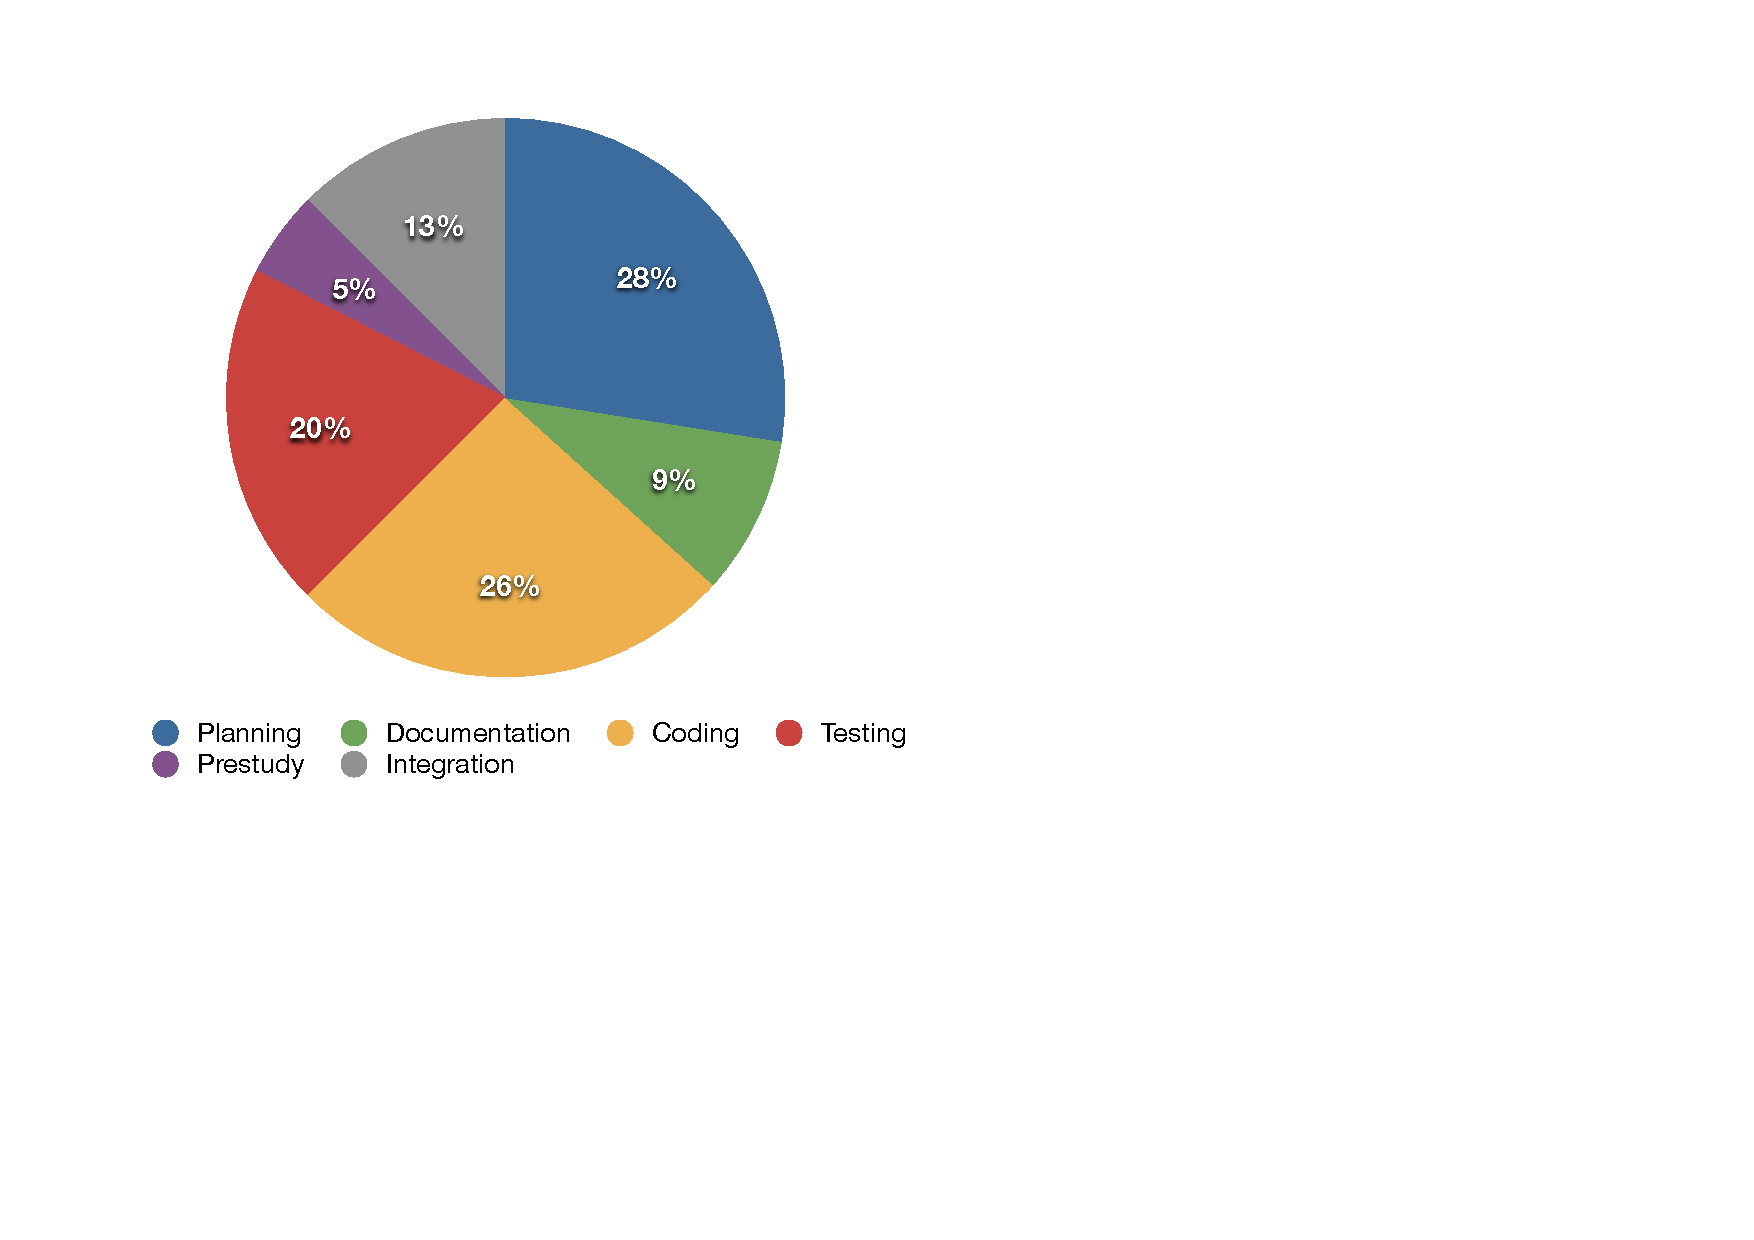
\includegraphics[scale=0.8]{img/pie_chart.pdf}
\caption{Story points breakdown}
\label{fig:sprints-points}
\end{figure}
